\section{基因组学概述}
\subsection{概述}
\begin{frame}
  \frametitle{基因组学 | 概述 | 基本概念}
  \begin{block}{基因}
基因(gene)是编码某种特定多肽链、tRNA、rRNA和ncRNA的DNA区段,是DNA上的功能单位。
  \end{block}
  \pause
  \begin{block}{基因组}
 基因组(genome)是一种生物体或个体细胞所具有的一套完整的基因及其调控序列 
  \end{block}
  \pause
  \begin{block}{基因组学}
 基因组学(genomics)是研究基因组的结构组成、时序表达模式和功能,并提供有关生物物种及其细胞功能的进化信息。 
  \end{block}
\end{frame}

\begin{frame}
  \frametitle{基因组学 | 概述 | 基本概念}
  \begin{figure}
    \centering
    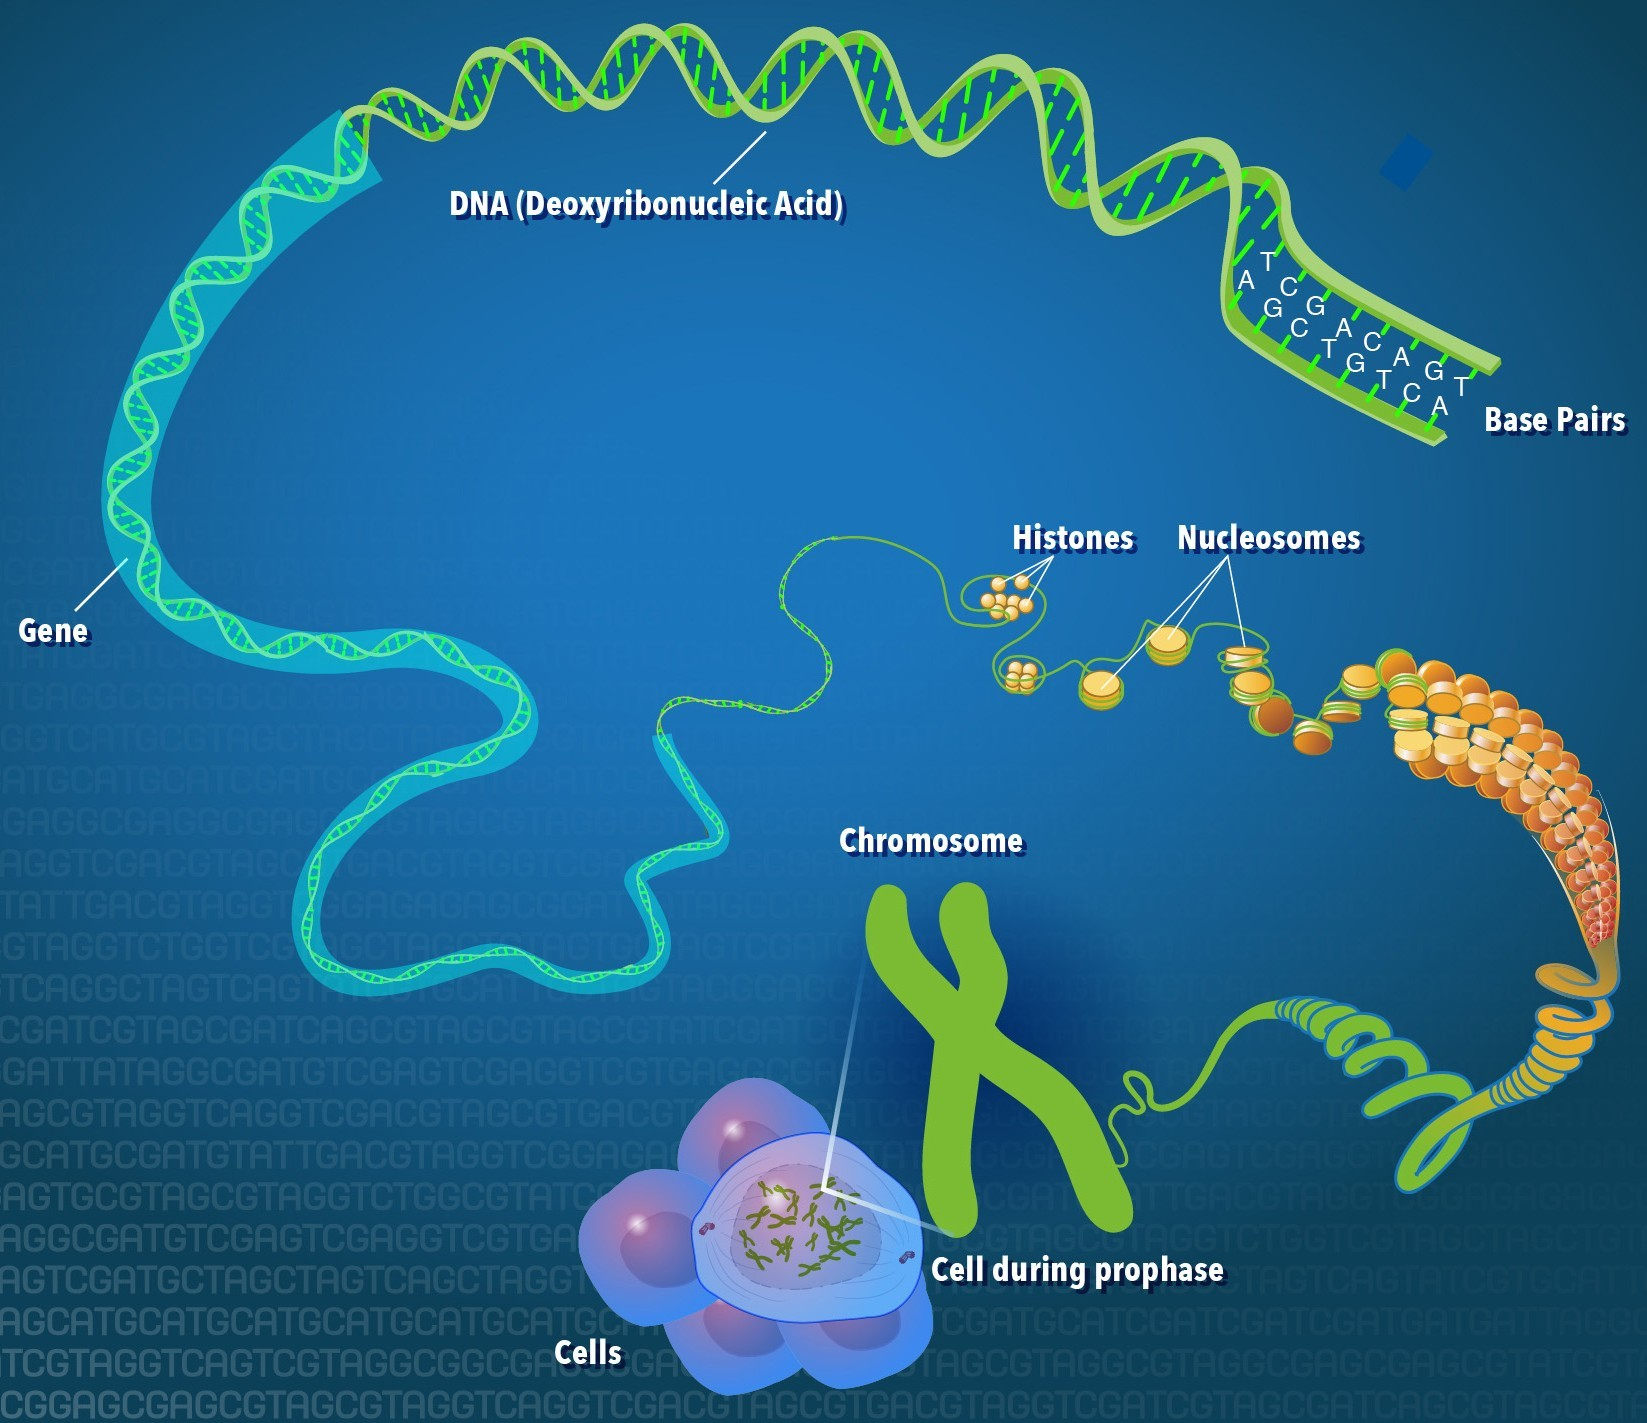
\includegraphics[width=0.7\textwidth]{c2.genomics/gene.01.jpg}
  \end{figure}
\end{frame}

\begin{frame}
  \frametitle{基因组学 | 概述 | 基因}
基因一词来自希腊语,意思为“生”。是指携带有遗传信息的DNA序列,是控制性状的基本遗传单位,亦即一段具有功能性的DNA序列。基因通过指导蛋白质的合成来表现所携带的遗传信息,从而控制生物个体的性状(差异)表现。人类约有两万至两万五千个基因。\\
\vspace{1em}
染色体在体细胞中是成对存在的,每条染色体上都带有一定数量的基因。一个基因在细胞有丝分裂时有两个对应的位点,称为等位基因,分别来自父与母。依所携带性状的表现,又可分为显性基因和隐性基因。\\
\vspace{1em}
一般来说,同一生物体中的每个细胞体都含有相同的基因,但并不是每个细胞中的所有基因携带的遗传信息都会被表现出来。职司不同功能的细胞中,活化而表现的基因也不同。
\end{frame}

\begin{frame}
  \frametitle{基因组学 | 概述 | 基因组}
在生物学中,一个生物体的基因组是指包含在该生物的DNA(部分病毒是RNA)中的全部遗传信息,又称基因体(genome)。基因组包括基因和非编码DNA。1920年,德国汉堡大学植物学教授汉斯·温克勒(Hans Winkler)首次使用基因组这一名词。\\
\vspace{1em}
更精确地讲,一个生物体的基因组是指一套染色体中的完整的DNA序列。例如,生物个体体细胞中的二倍体由两套染色体组成,其中一套DNA序列就是一个基因组。基因组一词可以特指整套核DNA(例如,核基因组),也可以用于包含自己DNA序列的细胞器基因组,如粒线体基因组或叶绿体基因组。当人们说一个有性生殖物种的基因组正在测序时,通常是指测定\textcolor{red}{一套常染色体和两种性染色体}的序列,这样来代表可能的两种性别。即使在只有一种性别的物种中,“一套基因组序列”可能也\textcolor{red}{综合了来自不同个体的染色体}。通常使用中,“遗传组成”一词有时在交流中即指某特定个体或物种的基因组。对相关物种全部基因组性质的研究通常被称为基因组学,该学科与遗传学不同,后者一般研究单个或一组基因的性质。
\end{frame}

\begin{frame}
  \frametitle{基因组学 | 概述 | 基因组}
对于像人类这样的脊椎动物,基因组通常指的只是染色体DNA。因此,尽管人类线粒体里包含了基因,但这些基因并不作为基因组的一部分。事实上,有时候称线粒体拥有自己的基因组,通常叫做\textcolor{red}{线粒体基因组}。而在叶绿体中的被称为\textcolor{red}{叶绿体基因组}。
\end{frame}

\begin{frame}
  \frametitle{基因组学 | 概述 | 基因组 | 测序}
  \begin{itemize}[<+->]
    \item 1976年,瓦尔特·菲尔斯(比利时根特大学)RNA病毒噬菌体MS2【第一个完整测序的基因组】
    \item 1977年,弗雷德里克·桑格,Φ-X174噬菌体【第一个完成测序的DNA基因组】
    \item 1995年,The Institute for Genomic Research团队,流感嗜血杆菌(\textit{Haemophilus influenzae})【第一个被测序的细菌基因组】
    \item 1996年,酿酒酵母(\textit{Saccharomyces cerevisiae})【第一个真核生物基因组】
    \item 1996年,The Institute for Genomic Research团队,詹氏甲烷球菌(\textit{Methanococcus jannaschii})【第一个被测序的古菌基因组】
    \item 1998年,秀丽隐杆线虫(\textit{Caenorhabditis elegans})【第一个被测序的多细胞生物基因组】
    \item 1990年,人类基因组计划启动
    \item 2007年,完成了詹姆斯·杜威·沃森个人基因组的测序
  \end{itemize}
\end{frame}

\begin{frame}
  \frametitle{基因组学 | 概述 | 基因组 | 补遗}
  \begin{block}{基因组构成}
基因组构成(genome composition)用于描述一个单倍体基因组的组成,包括基因组大小、非重复DNA和重复DNA所占的比重等。\\
\vspace{1em}
当讨论基因组的构成时,首先要区别的是原核基因组还是真核基因组,两者在基因组组成上有很大的不同。
  \end{block}
  \pause
  \begin{block}{基因组大小}
基因组大小是指一种生物单倍体基因组的全部DNA碱基对数。\\
\vspace{1em}
在原核生物和低等真核生物中,基因组大小与生物形态的复杂性基本呈正相关关系;但是在软体动物以及其它更高等的真核生物中,这种相关性就不存在了。这一现象可能是由基因组中的重复DNA引起的。 
  \end{block}
\end{frame}

\begin{frame}
  \frametitle{基因组学 | 概述 | 基因组 | 补遗}
  \begin{figure}
    \centering
    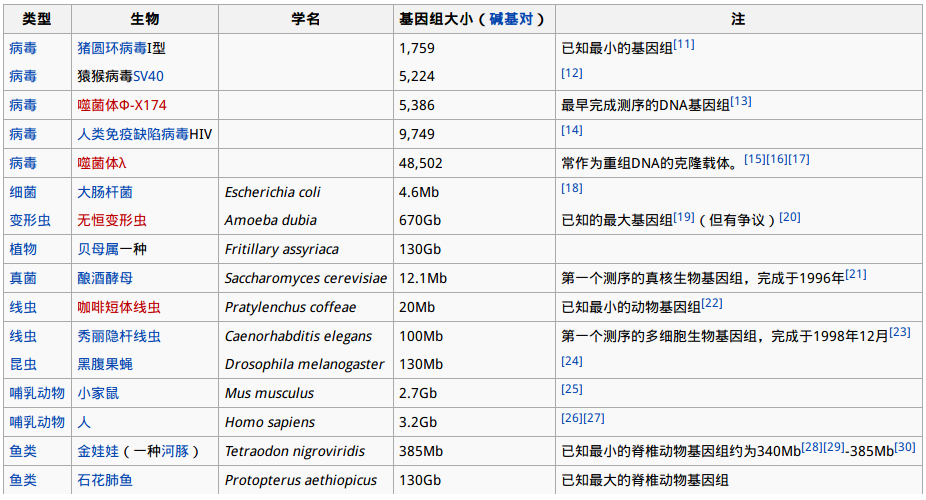
\includegraphics[width=\textwidth]{c2.genomics/genome.01.png}
  \end{figure}
\end{frame}

\begin{frame}
  \frametitle{基因组学 | 概述 | 基因组 | 补遗}
  \begin{block}{非重复DNA}
非重复DNA的总长除以基因组大小即为非重复DNA比重。蛋白质编码基因和非编码RNA基因一般都是非重复的DNA。\\
\vspace{1em}
不同生物中的非重复DNA的比重会有很大不同。更大的基因组并不意味着更多的基因,随着高等真核生物的基因组大小的增加,非重复DNA的比重相应减少。
  \end{block}
  \pause
  \begin{block}{基因组演化}
基因组不仅仅是是生物基因的集合,对其研究和比较能获得生物演化信息的更多细节。一些基因组性质如“染色体数”(核型)、基因组大小、基因顺序、密码子偏好性与GC含量能反映出现存生物的许多基因组演化信息。
  \end{block}
\end{frame}

\begin{frame}
  \frametitle{基因组学 | 概述 | 基因组学}
  \begin{block}{基因组学}
基因组学(genomics),或基因体学,是研究生物基因组和如何利用基因的一门学问。\\
\vspace{0.5em}
基因组学的主要工具和方法包括:生物信息学,遗传分析,基因表达测量和基因功能鉴定。
  \end{block}
  \pause
  \begin{block}{特点}
基因组学的特点是强调进行细胞中全部基因及非编码区的整体性考查和系统性研究,从而全面揭示基因与基因间的相互关系、基因与非编码序列的关系、基因与基因组的相互关系。
  \end{block}
\end{frame}

\begin{frame}
  \frametitle{基因组学 | 概述 | 基因组学}
  \begin{block}{组学}
“组”在基因组一词中,意指一个物种的“全部”遗传组成。由于诸如基因组测序这样的大规模定量生物项目的成功,“组”的这个意义的使用已经扩展到其他相关领域。例如,蛋白质组指的是一个物种组织或细胞内的全部蛋白质。 
  \end{block}
  \pause
  \begin{block}{基因组分析}
基因组项目涉及三个部分:DNA测序,该序列的组件生成原有染色体的表示法,以及该表示法的注释和分析。
  \end{block}
\end{frame}

\begin{frame}
  \frametitle{基因组学 | 概述 | 基因组学}
  \begin{itemize}[<+->]
    \item 1980年,噬菌体Φ-X174(5,368碱基对)完全测序,成为第一个测定的基因组
    \item 1995年,嗜血流感菌(Haemophilus influenzae,1.8Mb)测序完成,是第一个测定的自由生活物种
    \item 2001年,人类基因组计划公布了人类基因组草图,为基因组学研究揭开新的一页
    \item 2012年,千人基因组计划
  \end{itemize}
\end{frame}

\subsection{人类基因组计划}
\begin{frame}
  \frametitle{基因组学 | 概述 | 人类基因组}
  \begin{block}{人类基因组}
人类基因组,又称人类基因体,是智人的基因组,由\textcolor{red}{23对染色体}组成,其中包括\textcolor{red}{22对体染色体、1条X染色体和1条Y染色体}。人类基因组含有\textcolor{red}{约30亿个DNA碱基对},碱基对是以氢键相结合的两个含氮碱基,以胸腺嘧啶(T)、腺嘌呤(A)、胞嘧啶(C)和鸟嘌呤(G)四种碱基排列成碱基序列,其中A与T之间由两个氢键连接,G与C之间由三个氢键连接,碱基对的排列在DNA中也只能是A对T,G对C。其中一部分的碱基对组成了\textcolor{red}{大约20000到25000个基因}。 
  \end{block}
\end{frame}

\begin{frame}
  \frametitle{基因组学 | 概述 | 人类基因组}
  \begin{figure}
    \centering
    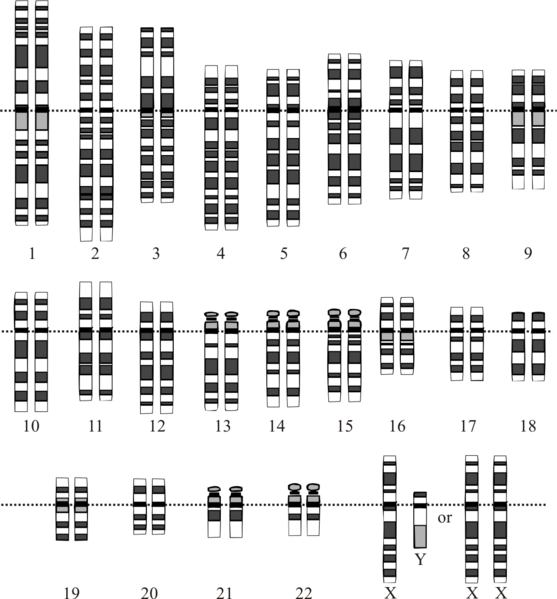
\includegraphics[width=0.6\textwidth]{c2.genomics/human.genome.01.png}
  \end{figure}
\end{frame}

\begin{frame}
  \frametitle{基因组学 | 概述 | 人类基因组 | 补遗}
  \begin{block}{染色体}
人类拥有23对不同的染色体,其中22对属于常染色体,另外还有1对能够决定性别的性染色体,分别是X染色体与Y染色体。1号到22号染色体的编号顺序,大致符合他们由大到小的尺寸排列。最大的染色体约含有2亿5千万个碱基对,最小的则约有3800万个碱基对。\\
\vspace{1em}
在人类个体的体细胞中,通常含有来自亲代的1到22对体染色体,再加上来自母亲的X染色体,以及来自父亲的X或Y染色体,总共是46个(23对)染色体。科学家将这些染色体分为7组:1号到3号是A组;4号与5号是B组;X染色体以及6号到12号是C组;13号到15号是D组;16号到18号是E组;19号与20号是F组;21号、22号与Y染色体是G组。对于一般人类来说,每个细胞核内只有两套染色体。
  \end{block}
\end{frame}

\begin{frame}
  \frametitle{基因组学 | 概述 | 人类基因组 | 补遗}
  \begin{block}{基因}
人体内估计约有20000到25000个蛋白质编码基因。虽然人类的基因数量比起某些较为原始的生物(如线虫与果蝇)更少,但是在人类细胞中使用了大量的选择性剪接(alternative splicing),这使得一个基因能够制造出多种不同的蛋白质,且人类的蛋白质组规模也较前述的两个物种更庞大。\\
\vspace{1em}
大多数人类基因拥有许多的外显子,且人类的内含子比位在其两端的外显子更长。这些基因参差不齐地分布在染色体中,每一个染色体皆含有一些基因较多的区段与基因较少的区段。这些区段的差异,则与染色体带(chromosome bands)及GC含量相关。基因密度所显现的非随机模式之涵义与重要性尚未明了。
  \end{block}
\end{frame}

\begin{frame}
  \frametitle{基因组学 | 概述 | 人类基因组 | 补遗}
  \begin{figure}
    \centering
    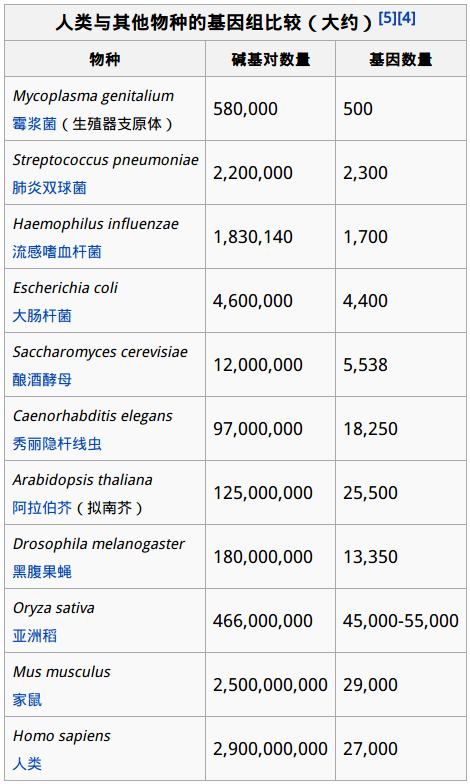
\includegraphics[width=0.38\textwidth]{c2.genomics/genome.size.01.png}
  \end{figure}
\end{frame}

\begin{frame}
  \frametitle{基因组学 | 概述 | 人类基因组 | 补遗}
  \begin{block}{功能未知区域}
    蛋白质编码序列(也就是外显子)在人类基因组中少于1.5\%。在基因与调控序列之外,仍然有许多功能未知的广大区域。科学家估计这些区域在人类基因组中约占有97\%,其中许多是属于重复序列(en:Repeated sequence (DNA))、转位子(transposon)与伪基因(pseudogene)。除此之外,还有大量序列不属于上述的已知分类。 \textcolor{red}{人类基因组内大量功能未知的序列,是目前科学研究的重点之一}。
  \end{block}
\end{frame}

\begin{frame}
  \frametitle{基因组学 | 概述 | 人类基因组 | 补遗}
  \begin{block}{变异}
    大多数对于人类遗传变异的研究集中在\textcolor{red}{单核苷酸多态性(single nucleotide polymorphisms;SNPs)},也就是DNA中的个别碱基变换。在人类的真染色质(富含基因的染色质)中,平均每100到1000个碱基会出现1个SNPs,不过密度并不均匀。由于SNPs的存在,如“所有人类的基因有99\%都是相同的”这样的说法并不精确。国际人类基因组单体型图计划(International HapMap Project),便是为了要将人类基因组中的SNP变异作编录,而组成的一个大规模合作计划。\\
\vspace{1em}
研究人员发现在人类与其他哺乳类DNA序列中的\textcolor{red}{拷贝数变异(copy number variation;CNV)},可能非常重要。拷贝数变异又称为拷贝数多型性(copy number polymorphisms;CNPs),是缺失(deletion)、插入(insertion)、重复(duplication),以及复杂多位置变异(complex multi-site variants)的合称,在所有人类以及其他已测试的哺乳动物中皆可发现。
  \end{block}
\end{frame}

\begin{frame}
  \frametitle{基因组学 | 概述 | 人类基因组 | 补遗}
  \begin{block}{演化}
比较基因组学(Comparative genomics)对于哺乳类基因组的研究显示,人类与大约两亿年前就已经分化的各物种相比,有大约5\%的比例在人类基因组中保留了下来,其中包含许多的基因与调控序列。而且人类与大多数已知的脊椎动物间,也享有了一些相同的基因。\\
 \vspace{1em}
黑猩猩的基因组与人类的基因组之间,有98.77\%是相似的。而平均每一个属于人类的标准蛋白质编码基因,只与属于黑猩猩的同源基因相差两个氨基酸;并且有将近三分之一的人类基因与黑猩猩的同源基因,能够翻译出相同的蛋白质。人类的2号染色体,是人类与黑猩猩基因组之间的主要差异,它是由黑猩猩的染色体12号与13号融合而成的。\\
 \vspace{1em}
人类在最近的演化过程中失去了嗅觉受体基因,这解释了为何人类比起其他的哺乳动物来说,拥有较差的嗅觉。演化上的证据显示,人类与某些灵长类所拥有的彩色视觉,降低了这些物种对于嗅觉能力的需求。
  \end{block}
\end{frame}

\begin{frame}
  \frametitle{基因组学 | 概述 | 人类基因组 | 补遗}
  \begin{block}{线粒体基因组}
大多数的基因是存在细胞核中,但是细胞中一个称为线粒体的细胞器,也拥有自己的基因组。线粒体基因组在线粒体疾病(mitochondrial disease)中具有一定的重要性;而且这些基因也可以用来研究人类的演化。线粒体位于细胞质中,当人类的精子与卵子结合时,源自母亲(女性)的卵子提供了绝大多数的细胞质,因此人类细胞中的线粒体基因皆是来自母亲。\\
\vspace{1em}
由于线粒体缺乏用来检查复制错误的能力,因此\textcolor{red}{线粒体DNA(mDNA)}的变异速率比细胞核DNA(一般所指的DNA)更快。线粒体的突变速率快了20倍,这使mDNA能够用来较为精确地追溯出母系祖先。研究族群中的mDNA,也能使人们得知此族群过去的迁移路径。
  \end{block}
\end{frame}

\begin{frame}
  \frametitle{基因组学 | 概述 | 人类基因组计划}
  \begin{figure}
    \centering
    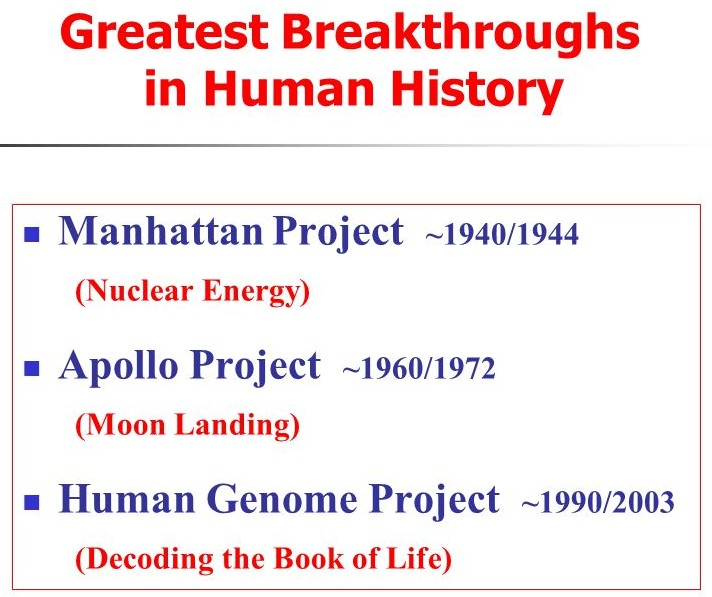
\includegraphics[width=0.7\textwidth]{c2.genomics/hgp.01.jpg}
  \end{figure}
\end{frame}

\begin{frame}
  \frametitle{基因组学 | 概述 | 人类基因组计划}
人类基因组计划(human genome project, HGP)是一项规模宏大,跨国跨学科的科学探索工程。其宗旨在于测定组成人类染色体(指单倍体)的30亿个碱基对形成的核苷酸序列,从而绘制人类基因组图谱,并且辨识其载有的基因,达到破译人类遗传信息的最终目的。\\
\vspace{1em}
该计划起始于1990年,已基本测序了人类的所有基因。截止到2005年,人类基因组计划的测序工作已经基本完成(92\%)。但关于其功能的细节,则仍有许多研究在进行中。\\
\vspace{1em}
其中,2001年人类基因组工作草图的发表被认为是人类基因组计划成功\textcolor{red}{【?】}的里程碑。
\end{frame}

\begin{frame}
  \frametitle{基因组学 | 概述 | 人类基因组计划 | 事件}
  \begin{itemize}[<+->]
    \item 1984年,第一次讨论人类基因组测序的价值
    \item 1985年,首次对于人类基因组测序的可行性进行认真的探讨
    \item 1986年,罗纳德·杜尔贝科(Renato Dulbecco),建议开展人类基因组研究计划
    \item 1986年,美国能源部(DOE)加入人类基因组计划
    \item 1987年,美国国家卫生研究院(NIH)加入人类基因组计划
    \item 1998年,詹姆士·华生,NIH的基因组部门主管(1988-1992)
    \item 1988年,国际人类基因组组织(HUGO)成立
  \end{itemize}
\end{frame}

\begin{frame}
  \frametitle{基因组学 | 概述 | 人类基因组计划 | 事件(续)}
  \begin{itemize}[<+->]
    \item 1990年,投资30亿美元的人类基因组计划由美国能源部和国家卫生研究院正式启动,预期在15年内完成,随后扩展为国际合作的人类基因组计划
    \item 1996年,百慕大会议,以2005年完成测序为目标,分配了各国负责的工作,并且宣布研究结果将会即时公布,且完全免费
    \item 1998年,克莱格·凡特的塞雷拉基因组公司成立,希望能以更快的速度和更少的投资(3亿美元)来完成此项工程;开发出全世界第一台全自动测序仪,宣布将在2001年完成测序工作
    \item 2000年6月26日,塞雷拉公司的代表凡特,以及国际合作团队的代表弗朗西斯·柯林斯(Francis Collins),在美国总统克林顿的陪同下发表演说,宣布人类基因组的概要已经完成;所有人类基因组数据为人类共同财产,不允许专利保护,且必须对所有研究者公开
    \item 2001年2月,国际人类基因组测序联盟与塞雷拉公司,分别将研究成果发表于《自然》与《科学》;覆盖基因组序列的83%,包括常染色质区域的90%(带有150,000个空缺,且许多片断的顺序和方位并没有得到确定)
  \end{itemize}
\end{frame}

\begin{frame}
  \frametitle{基因组学 | 概述 | 人类基因组计划 | 事件 | 中国}
  \begin{itemize}[<+->]
    \item 1994年,中国的人类基因组计划启动
    \item 1998年,中国南方基因组中心成立,中国科学院遗传研究所人类基因组中心成立
    \item 1999年,北京华大基因研究中心(华大基因)成立,北方基因组中心成立
    \item 1998年3月,中美港科学家合作,成功地将与华人和鼻咽癌有关的肿瘤抑制基因定位于人类第3号染色体的短臂3p21.3位点
    \item 1999年6月26日,中国科学院遗传研究所人类基因组中心向美国国立卫生研究院(NIH)的国际人类基因组计划(HGP)递交加入申请。HGP在网上公布中国注册加入国际测序组织,中国成为继美、英、日、德、法后第六个加入该组织的国家
    \item 1999年11月10日,1\%计划被列入中国国家项目,并确定由北京华大基因研究中心(华大基因)牵头,国家基因组南方中心、北方中心共同参与,承担全部工程1%的测序工作
    \item 2000年4月,中国完成了人第3号染色体上3000万个碱基对的工作草图
  \end{itemize}
\end{frame}

\begin{frame}
  \frametitle{基因组学 | 概述 | 人类基因组计划 | 事件}
  \begin{figure}
    \centering
    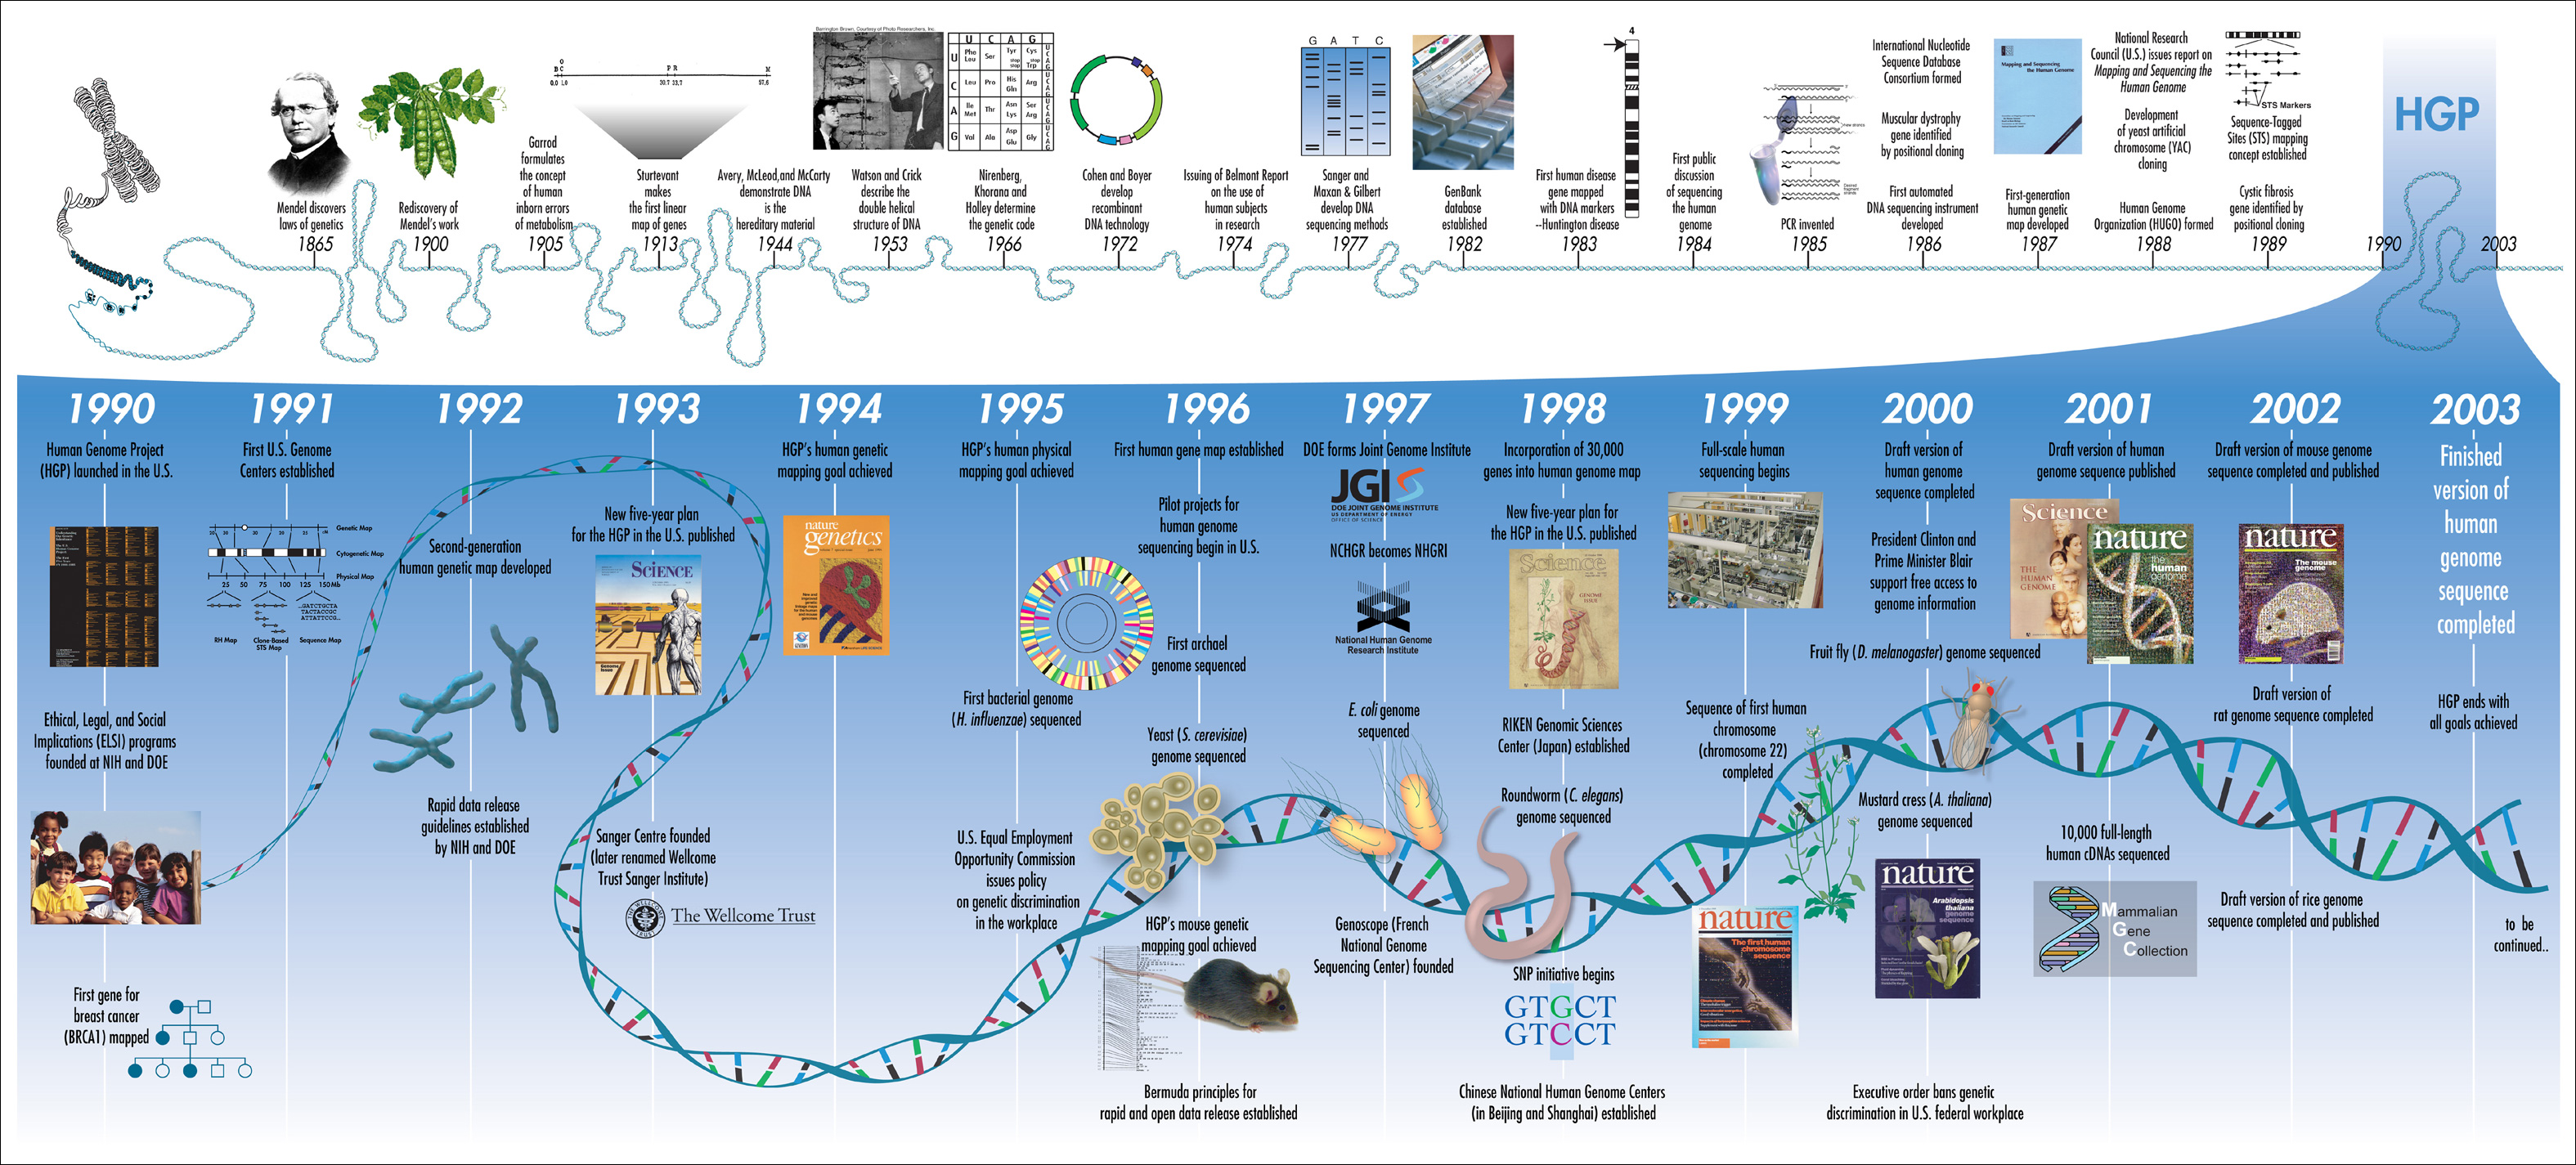
\includegraphics[width=\textwidth]{c2.genomics/hgp.timeline.01.jpg}
  \end{figure}
\end{frame}

\begin{frame}
  \frametitle{基因组学 | 概述 | 人类基因组计划 | 目标}
  \begin{description}[<+->]
    \item[遗传图谱的绘制] 遗传图谱主要是用遗传标签来确定基因在染色体上的排列。 
    \item[物理图谱的绘制] 物理图谱是通过序列标签位点对构成基因组的DNA分子进行测定,从而对某基因所相对之遗传讯息及其在染色体上的相对位置做一线性排列。
    \item[序列测定] 通过测序得到基因组的序列,是一般意义上的人类基因组计划。 
    \item[辨别序列中的个体差异] 人类基因组计划只是为未来鉴定不同个体间基因组差异做一些基础的框架性工作。当前主要工作在于鉴定不同个体间包含的单核苷酸多态性。
    \item[基因鉴定] 以获得全长的人类cDNA文库为目标。
    \item[基因的功能性分析] 对海量的数据进行标注,分析注释序列。另一个目标是研发出更快更有效的方法来进行DNA测序和序列分析,并把这一技术加以产业化。 
  \end{description}
\end{frame}

\begin{frame}
  \frametitle{基因组学 | 概述 | 人类基因组计划 | 目标 | 完成情况}
  \begin{description}[<+->]
    \item[遗传图谱的绘制] 1994年9月,完成了包含3000个(原计划为600-1500)标签分辨率为1-cM(即1\%重组率)的遗传图谱的绘制。
    \item[物理图谱的绘制] 1998年10月,完成了包含52,000个(原计划为30,000)序列标签位点的物理图谱的绘制。
    \item[序列测定] 2003年4月,包含基因序列中的98%(原预计为95%)获得了测定,精确度为99.99%。
    \item[辨别序列中的个体差异] 至2003年2月,已有约3,700,000个单核苷酸多态性位点得到测定。
    \item[基因鉴定] 至2003年3月,已获得15,000个全长的人类cDNA文库。
    \item[基因的功能性分析] 已获得开发的技术包括高通量寡聚核苷酸的合成(1994年)、DNA微阵列(1996年)、标准化和消减化cDNA文库(1996年)、真核(酵母)全基因组敲除技术(1999年)、大型化双杂交定位(2002年)。
  \end{description}
\end{frame}

\begin{frame}
  \frametitle{基因组学 | 概述 | 人类基因组计划 | 图谱}
  \begin{block}{遗传图谱}
遗传图谱(genetic map)是利用基因的重组率来做分析,单位是分莫甘(centimorgan)。这种图谱表现出来的是基因或特定DNA片段之间的相对位置,而不是它们各自的绝对位置。
  \end{block}
  \pause
  \begin{block}{物理图谱}
物理图谱(physical map)则是DNA两点的实际距离,是实际将DNA片段排序而得,单位是碱基的数目(如Kb;kilobase)。
  \end{block}
\end{frame}

\begin{frame}
  \frametitle{基因组学 | 概述 | 人类基因组计划 | 完成?}
  \begin{block}{完成}
关于如何界定人类基因组测序完成,有多种定义。根据不同的定义,人类基因组的测序是否完成有不同的看法。曾有多个大众媒体报道人类基因组计划“完成”,而且由国际人类基因组计划所采用的定义,基因组的测序已经完成。
  \end{block}
  \pause
  \begin{block}{仍有许多的区域未获得测序}
    \begin{itemize}
      \item 着丝粒含有数百万(可能接近千万)的碱基对,其中的大多数完全没有得到测序
      \item 染色体末端区域(称为端粒)大都不完整,无法精确地知道在端粒前还有多少序列
      \item 每个人的基因组中都含有多个包含多基因家族成员的位点
      \item 还有一些间隙散布于基因组中,部分间隙较大
    \end{itemize}
  \end{block}
\end{frame}

\begin{frame}
  \frametitle{基因组学 | 概述 | 人类基因组计划 | 意义}
  \begin{itemize}
    \item 基础科研领域:癌症、老年痴呆症等疾病的病因研究,推动新的疗法和新药的开发研究
    \item 医疗健康/商业价值:基因检测,个性化医疗/精准医疗
    \item 生物进化研究:揭示了许多重要的生物进化史上的里程碑事件(核糖体的出现,器官的产生,胚胎的发育,脊柱和免疫系统等)
    \item 人类遗传信息的应用:考古学(走出非洲),犯罪学以及社会执法
  \end{itemize}
\end{frame}

\begin{frame}
  \frametitle{基因组学 | 概述 | 人类基因组计划 | 补遗}
  \begin{itemize}
    \item 2004年,国际人类基因组测序联盟的研究者宣布,人类基因组中所含基因的预计数目从先前的30,000至40,000(在计划初期的预计数目则高达2,000,000)调整为20,000至25,000。预期还需要多年的时间来确定人类基因组中所含基因的精确数目。
    \item 目前基因组信息的注释工作仍然处于初级阶段。
  \end{itemize}
\end{frame}

\begin{frame}
  \frametitle{基因组学 | 概述 | 人类基因组计划 | 补遗}
  \begin{block}{延伸计划}
    \begin{description}
      \item[模式生物的基因组计划] 小鼠、果蝇、线虫、斑马鱼、酵母等
      \item[人类元基因组计划] 对人体内所用共生菌群的基因组进行序列测定,并研究与人体发育和健康相关基因的功能
      \item[国际人类基因组单体型图计划(HapMap计划)] 目标是构建人类DNA序列中多态位点的常见模式,为研究人员确定对健康和疾病以及对药物和环境反应有影响的相关基因提供关键信息 
      \item[人类基因组多样性研究计划] 对不同人种、民族、人群的基因组进行研究和比较,这一计划将为疾病监测、人类的进化研究和人类学研究提供重要信息
      \item[千人基因组计划(1000 Genomes Project)] 目标是建立最详尽的人类遗传变异目录。启动于2008年1月,计划在随后三年内,测定来自不同族群的数量至少一千名的匿名参与者的基因组序列。2010年完成试点阶段,2012年10月公布1092个基因组的测序
    \end{description}
  \end{block}
\end{frame}

\subsection{分支学科}
\begin{frame}
  \frametitle{基因组学 | 概述 | 分支学科 | 结构基因组学}
  \begin{block}{结构基因组学}
结构基因组学(Structural Genomics)是基因组学的一个重要组成部分和研究领域,它是一门通过基因作图、核苷酸序列分析确定基因组成、基因定位的科学。
  \end{block}
\end{frame}

\begin{frame}
  \frametitle{基因组学 | 概述 | 分支学科 | 功能基因组学}
  \begin{block}{功能基因组学}
功能基因组学(Functional genomics)的研究又往往被称为后基因组学(Postgenomics)研究,它是利用结构基因组学提供的信息和产物,在基因组或系统水平上全面分析基因的功能和相互作用。\\
\vspace{1em}
功能基因组学是利用结构基因组学所获得的各种信息,建立与发展各种技术和实验模型来测定基因及基因非编码序列的生物学功能。
  \end{block}
\end{frame}

\begin{frame}
  \frametitle{基因组学 | 概述 | 分支学科 | 功能基因组学}
  \begin{figure}
    \centering
    
\includegraphics[width=0.65\textwidth]{c2.genomics/functional.genomics.02.jpg}
  \end{figure}
\end{frame}

\begin{frame}
  \frametitle{基因组学 | 概述 | 分支学科 | 比较基因组学}
  \begin{block}{比较基因组学}
比较基因组学(Comparative genomics)是在基因组图谱和测序技术的基础上,对已知的基因特征和基因组结构进行比较以了解基因的功能、表达机制和不同物种亲缘关系的生物学研究。比较基因组学的基础是相关生物基因组的相似性。全基因组比对是比较基因组学的经典方法。比较基因组学的研究成果催生了水平基因转移理论,支持细胞器起源的内共生学说。\\
\vspace{1em}
比较基因组学是研究比较不同物种基因组的异同,目的在于寻找物种间共有的、也就是在进化上保守的基因或DNA序列,这些基因往往具有重要的生物学功能。也可以从这些模式生物中寻找人类可能具有的新基因,以及为预测新的基因功能提供依据。
  \end{block}
\end{frame}

\begin{frame}
  \frametitle{基因组学 | 概述 | 分支学科 | 比较基因组学}
  \begin{figure}
    \centering
    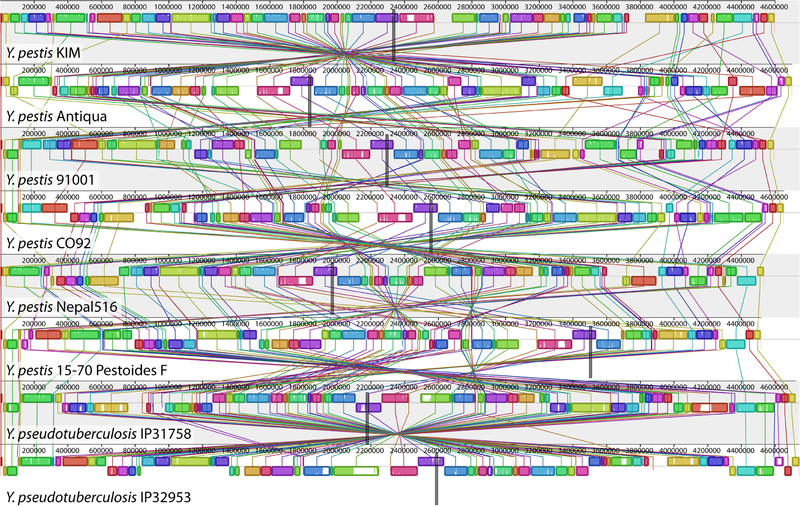
\includegraphics[width=0.9\textwidth]{c2.genomics/comparative.genomics.01.png}
  \end{figure}
\end{frame}

\begin{frame}
  \frametitle{基因组学 | 概述 | 分支学科 | 比较基因组学 | 种间}
  \begin{block}{种间比较基因组学研究}
通过对不同亲缘关系物种的基因组序列进行比较,能够鉴定出编码序列、非编码调控序列及给定物种独有的序列。而基因组范围之内的序列比对,可以了解不同物种在核苷酸组成、同线性关系和基因顺序方面的异同,进而得到基因分析预测与定位、生物系统发生进化关系等方面的信息。
  \end{block}
\end{frame}

\begin{frame}
  \frametitle{基因组学 | 概述 | 分支学科 | 比较基因组学 | 种内}
  \begin{block}{种内比较基因组学研究}
同种群体内基因组存在大量的变异和多态性,正是这种基因组序列的差异构成了不同个体与群体对疾病的易感性和对药物与环境因子不同反应的遗传学基础。
\begin{itemize}
  \item 单核苷酸多态性(single-nucleotide polymorphism,SNP)是指在基因组水平上由于单个核苷酸位置上存在转换或颠换等变异所引起的DNA序列多态性。
  \item 拷贝数多态性(copy number polymorphism,CNP):平均2个个体间存在11个CNP的差异,CNP的平均长度为465kb,其中半数以上的CNP在多个个体中重复出现,并经常定位于其他类型的染色体重排附近。
\end{itemize}
  \end{block}
\end{frame}

\begin{frame}
  \frametitle{基因组学 | 概述 | 分支学科 | 比较基因组学 | 研究方法}
  \begin{block}{系统发育谱法}
系统发育谱法(phylogenetic profile method)是在基因组全序列已完成测序的一系列基因组中分析某一蛋白质存在与否的模式。如果两个蛋白质在所研究的若干基因组中有相同的系统发育谱,便推断这两个蛋白质具有功能联系。
  \end{block}
  \pause
  \begin{block}{基因邻居法}
    基因邻居法(gene neighbour method)的原理是原核生物中如果两个基因在一个共同的操纵子内,且在不同的其他基因组也出现相邻现象,就可以推断它们编码的蛋白质之间具有功能联系。
  \end{block}
\end{frame}

\begin{frame}
  \frametitle{基因组学 | 概述 | 分支学科 | 比较基因组学 | 研究方法}
  \begin{figure}
    \centering
    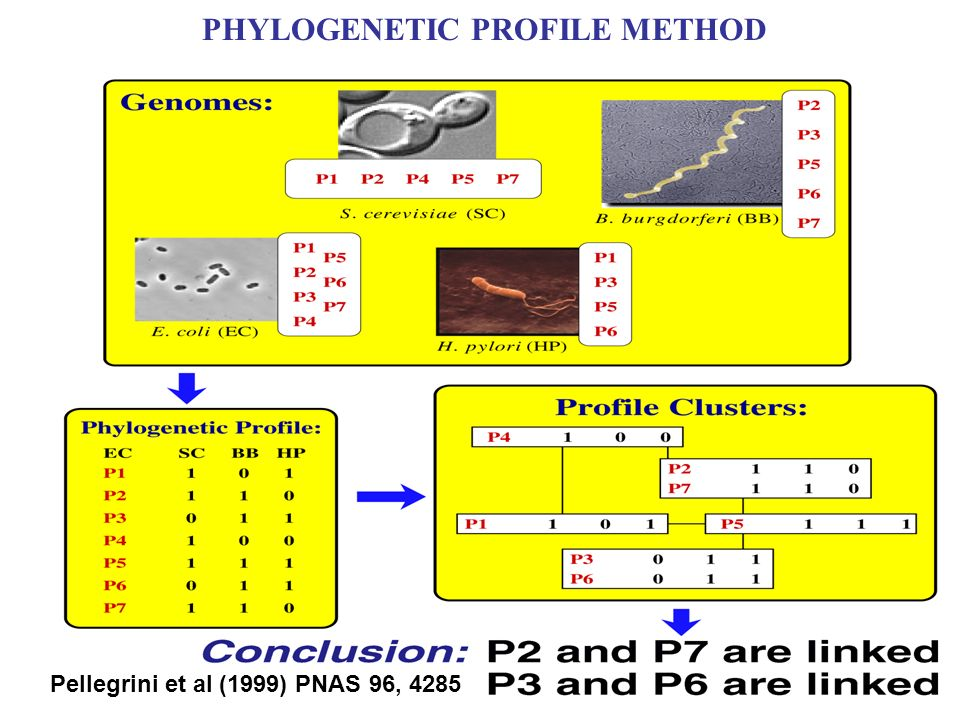
\includegraphics[width=0.9\textwidth]{c2.genomics/comparative.genomics.ppm.01.jpg}
  \end{figure}
\end{frame}

\begin{frame}
  \frametitle{基因组学 | 概述 | 分支学科 | 比较基因组学 | 研究方法}
  \begin{figure}
    \centering
    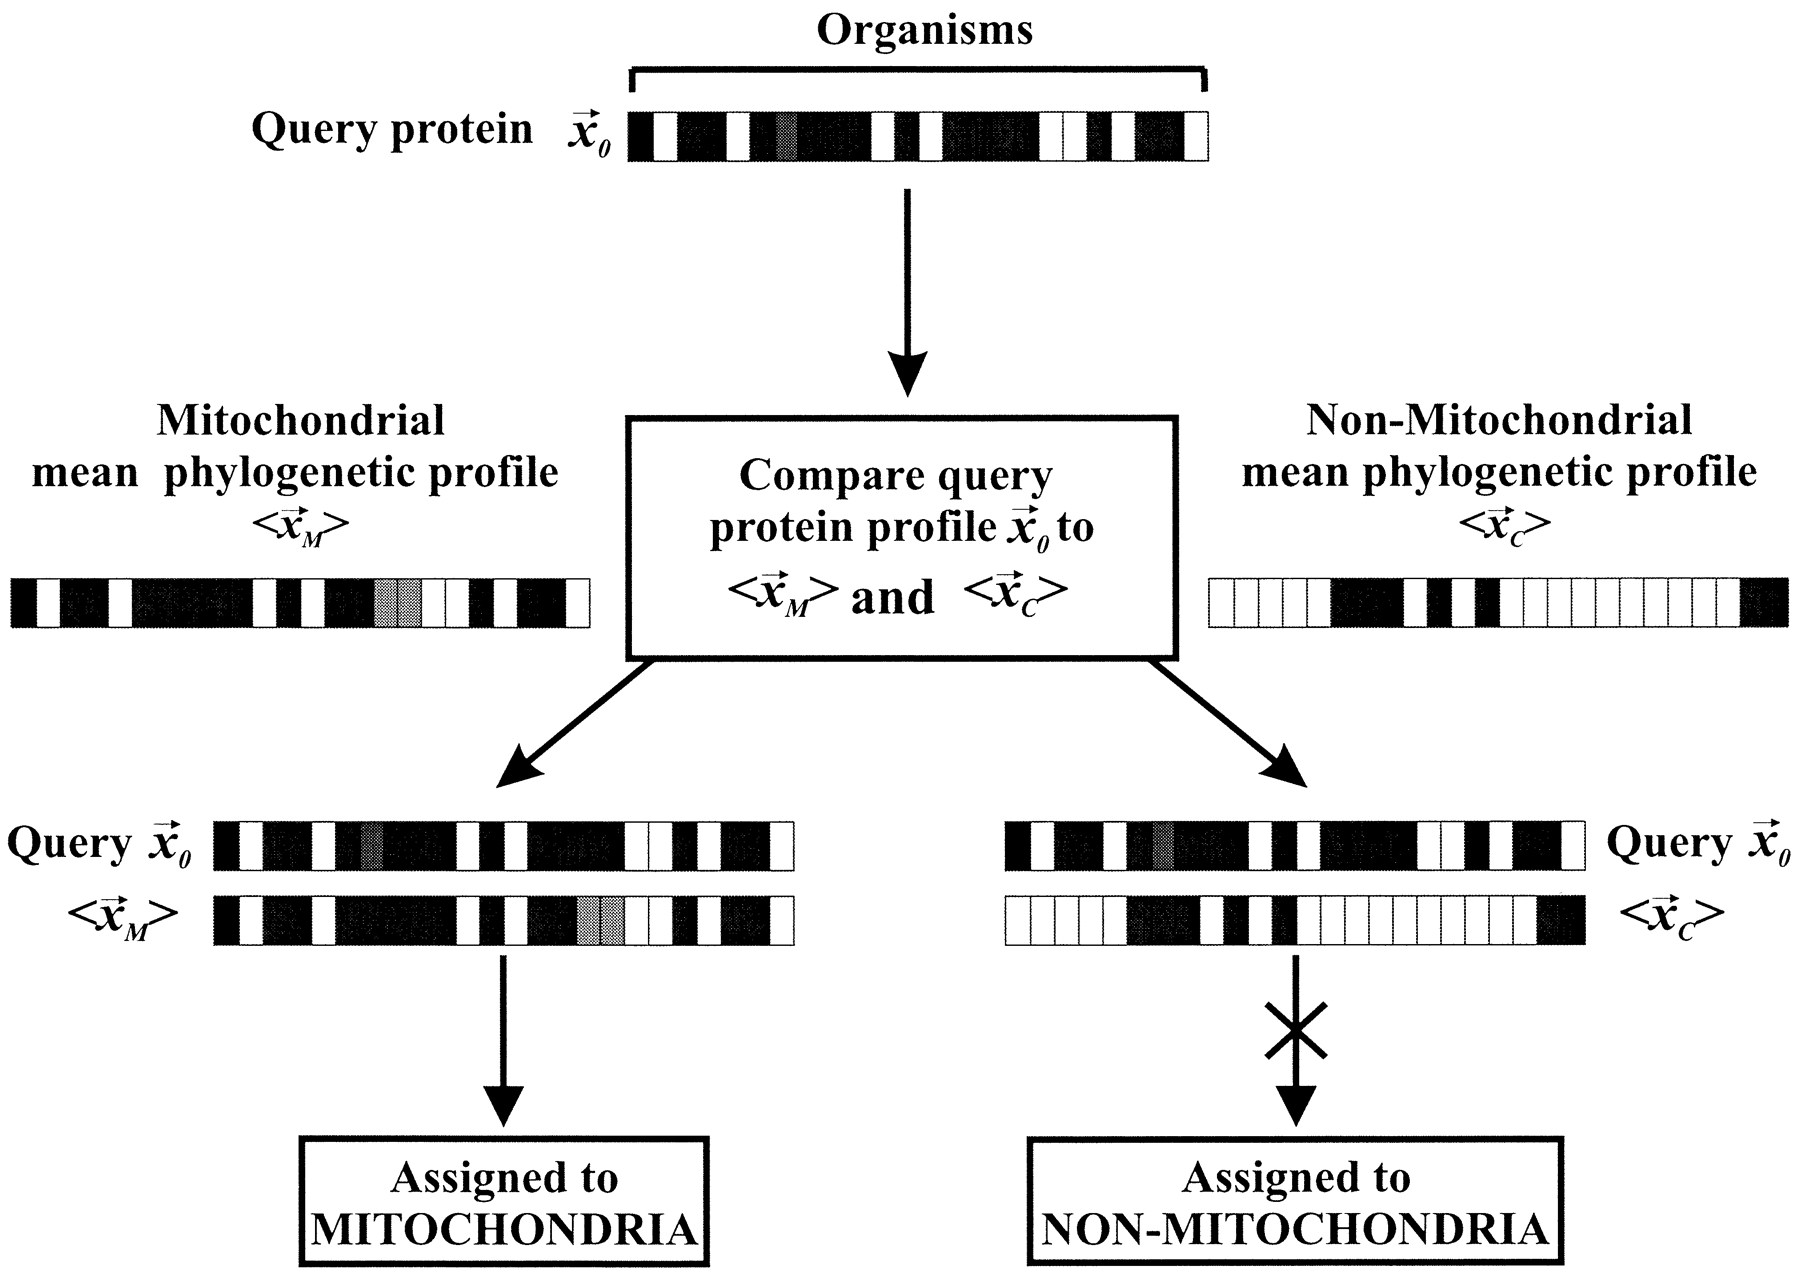
\includegraphics[width=0.9\textwidth]{c2.genomics/comparative.genomics.ppm.02.jpg}
  \end{figure}
\end{frame}

\begin{frame}
  \frametitle{基因组学 | 概述 | 分支学科 | 药物基因组学}
  \begin{block}{药物基因组学}
药物基因组学旨在理解个体对药物不同反应的遗传北京,即为什么某种药物对一部分人群有效,而对另一部分人群效果不佳或完全失效。\\
\vspace{1em}
制药业将充分应用药物基因组学的理论知识和技术手段来设计临床实验并模拟和分析理论与实验数据,也为新药设计和筛选提供依据。
  \end{block}
\end{frame}

\begin{frame}
  \frametitle{基因组学 | 概述 | 分支学科 | 药物基因组学}
  \begin{block}{个体对药物不同反应的遗传背景研究}
人类基因组DNA在个体间一般呈现0.01\%差异,几乎每个基因都有一个核苷酸变异谱。这是人类个体对药物敏感性不同的遗传基础,也是现代医学提出药物治疗必须个体化的依据。
  \end{block}
  \pause
  \begin{block}{为药物设计和筛选提供依据}
现代药物设计应考虑与遗传有关的若干因素:
\begin{itemize}
  \item 与致病有关的等位基因常会影响到对药物作用的反应
  \item 药物代谢途径与疗效密切相关
\end{itemize}
  \end{block}
\end{frame}

\begin{frame}
  \frametitle{基因组学 | 概述 | 分支学科 | 元基因组学}
  \begin{block}{元基因组学}
元基因组或总体基因组学(Metagenomics)是一门直接取得环境中所有遗传物质的研究,意指直接研究环境中微生物群落基因体学的应用,而非于实验室中进行单一个体纯化与培养的实验方式。研究领域广泛,也可称为环境基因组学、生态基因组学或群落基因组学。\\
\vspace{1em}
在早期研究微生物基因体必须将环境基因DNA或RNA克隆进入大肠杆菌体内,利用复制扩增方式,分析在自然环境中复制扩增特定基因(通常为16S rRNA)的多样性。但是,以复制扩增的方式得不到精准的微生物多样性。总体基因体学是认识复杂微生物群落的主要途径,提供一个更客观的方式发现微生物的世界,有可能改变之前我们所认知的微生物世界。
  \end{block}
\end{frame}

\begin{frame}
  \frametitle{基因组学 | 概述 | 分支学科 | 元基因组学}
  \begin{figure}
    \centering
    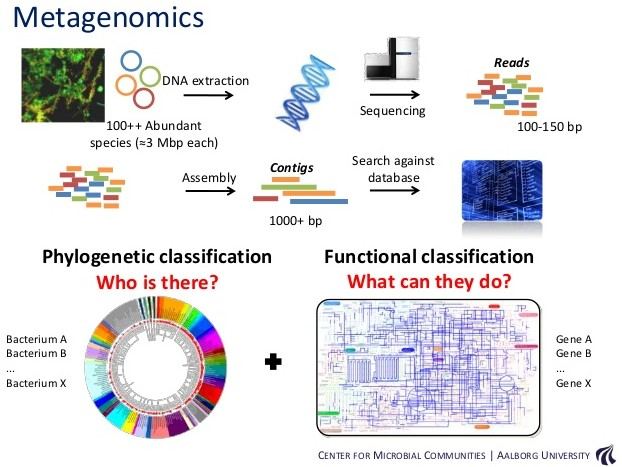
\includegraphics[width=0.8\textwidth]{c2.genomics/metagenomics.01.jpg}
  \end{figure}
\end{frame}

\begin{frame}
  \frametitle{基因组学 | 概述 | 分支学科 | 元基因组学 | 人体元基因组}
人类元基因组是指与人类共生的全部微生物的基因总和。又被称为“微生物组”或“人类第二基因组”。\\
\vspace{1em}
人类体内的微生物多达1000多种,特别是胃肠道内的微生物最为丰富;因此我们所说的元基因组在狭义上指的是肠道源基因组。\\
\vspace{1em}
人体内微生物的编码基因的总量大约是人类编码基因数目的50-100倍,这相当于在人类体内存在着另一个基因组通过表达调控人体的生命健康,即第二基因组。\\
\vspace{1em}
目前关于元基因组的研究还处于一个比较浅的阶段,在现有的研究中普遍认为糖尿病和肥胖症与人体元基因组有关。\\
\vspace{1em}
美国国立卫生研究院在2007年启动人体微生物计划,这计划一开始最主要的目的是调查是否有人体微生物的存在、了解人体微生物的变化与人类健康的关系,并开发新的技术和生物资讯的工具以支持这些目标。
\end{frame}

